\documentclass[11pt,a4paper]{article}

\usepackage[utf8]{inputenc} 
\usepackage[T1]{fontenc} 
\usepackage{lmodern}
\usepackage[margin=2cm]{geometry}
\usepackage[german]{babel}
\usepackage{amsmath} 
\usepackage{graphicx} 
\usepackage{booktabs}
\usepackage{hyperref}
\hypersetup{
    colorlinks,
    citecolor=red,
    filecolor=black,
    linkcolor=black!20!blue!90!,
    urlcolor=black} 
\usepackage{nicefrac}
\usepackage[table]{xcolor}
\usepackage{tocloft}
\usepackage{multirow}

\setlength{\parindent}{0pt}
\setlength{\parskip}{1ex plus 0.5ex minus 0.5ex}

\definecolor{incolor}{rgb}{0.0, 0.0, 0.5}

\hbadness=99999

\newcommand{\refpy}[1]{Siehe Anhang: \textit{Rechnungen in Python} (\texttt{{\color{incolor}In [{\color{incolor}#1}]}})}
\newcommand\dif{\mathop{}\!\mathrm{d}}
\newcommand{\halftime}[4]{\begin{figure}[h]
\begin{minipage}{.#1\textwidth}#3\end{minipage}\begin{minipage}{.#2\textwidth}
\centering
#4\end{minipage}
\end{figure}}


\begin{document}

{
\centering 
\large 
Physiklabor für Anf\"anger*innen \\
Ferienpraktikum im Sommersemester 2018 \\[4mm]
\textbf{\LARGE 
Versuch 19: Gekoppeltes Pendel 
} \\[3mm]
(durchgef\"uhrt am 19.09.2018 bei Adrian Hauber) \\
Gruppe 14: Andréz Gockel, Patrick M\"unnich\\
\today \\[10mm]
}

\vspace{50pt}
\tableofcontents
\vspace{22pt}
\listoftables
\vspace{22pt}
\listoffigures
\pagebreak

\section{Ziel des Versuchs}
Das Ziel dieses Versuchs ist einen gekoppelten Oszillator durch einen gekoppelten Pendel zu veranschaulichen. Hierzu werden erst die Differentialgleichungen hergeleitet und durch das Drehmoment entkoppelt, um die Eigenfrequenzen zu berechnen womit die Schwebungsdauer aus den Schwingungsdauern berechnet werden kann. In diesem Versuch werden Periodendauern bei verschiedenen Kopplungsgraden gemißt und zusätzlich die Schwebungsdauer. Der Kopplungsgrad wird verändert indem die Kopplungsfeder verschoben wird. Zusätzlich wird der Koppelungsgrad durch die Schwingdauern berechnet.

\section{Messung der Schwingungsdauern}

\subsection{Theorie}

Um den Koppelungsgrad zu bestimmen wird zunächst die Differentialgleichung des gekoppelten Pendels hergeleitet.
Das 

\subsection{Aufbau}

\halftime{5}{5}{In diesem Versuch haben wir zwei Pendel mit die aus einer festen Stange und einem Zusatzkörper bestehen. Eine Feder die beide Pendel koppelt hängt mit der verstellbaren Länge $l$ von dem Aufhängepunkt des Pendels. Vor beginn der Messungen ist zu beachten:
\begin{itemize}
	\item das der Aufbau komplett eben sein muss
	\item das beide Pendel mit gleicher Periodendauer schwingen
\end{itemize}
Unsere Kalibriermessung ergab $18.70(5)$\,s für 10 Schwingungen beider Pendel. % maybe formulate gooder
Die länge der Pendel von Aufhängepunkt zu der Masse ist jeweils $L = 95.0(5)$\,cm.
}{\fbox{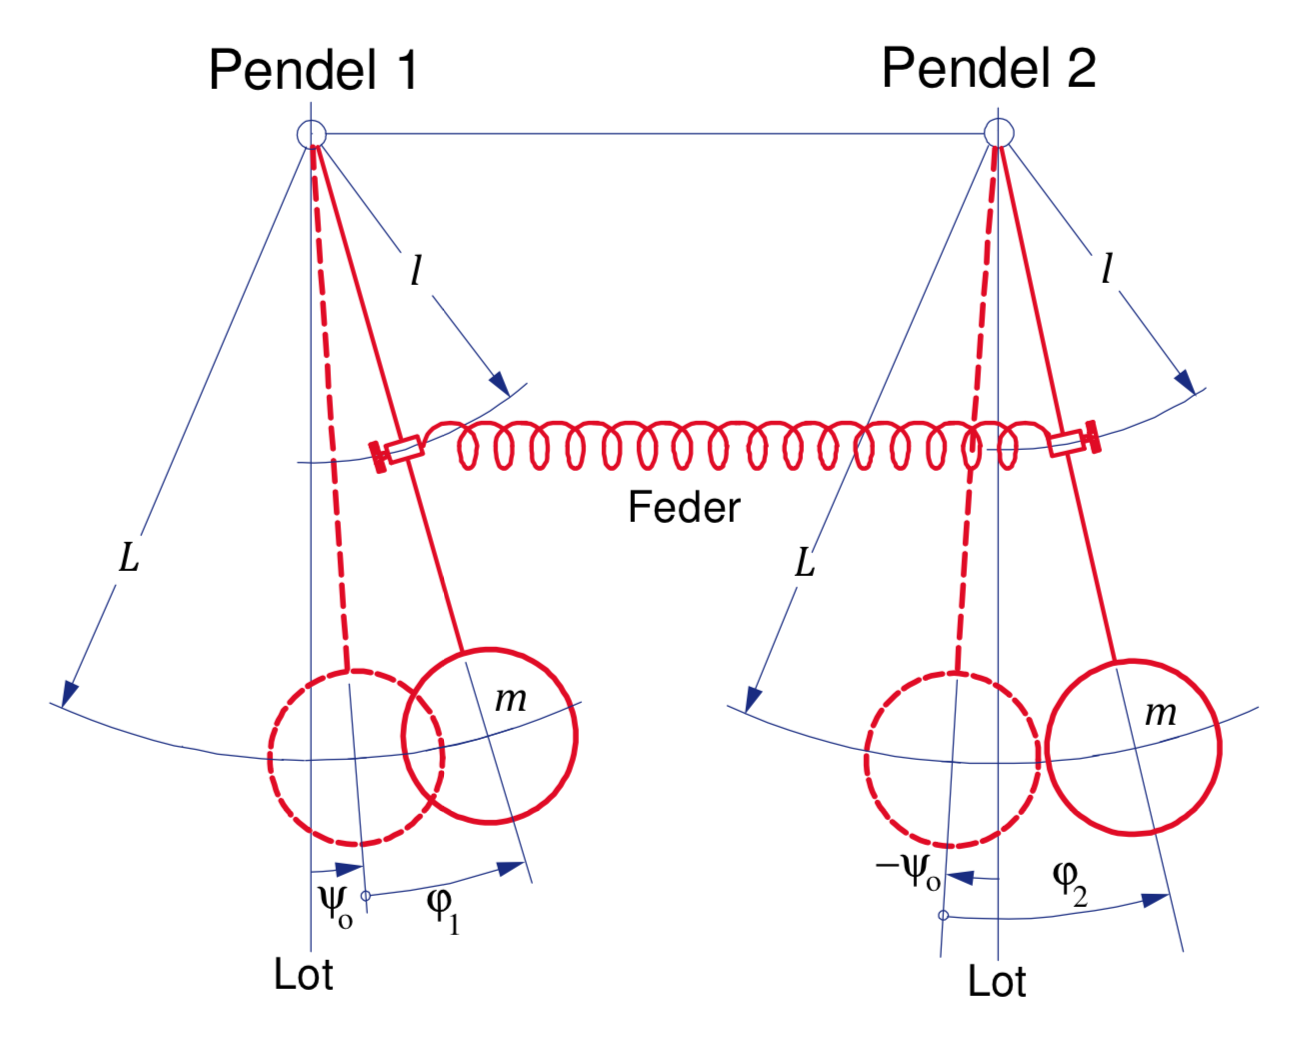
\includegraphics[width=0.9\textwidth]{ndp}}
   \renewcommand\thefigure{B1}
\caption[Gekoppeltes Pendel]{Gekoppeltes Pendel \cite{Anleitung}}
\label{Pic:1}}

\subsection{Durchführung}

Wir haben zuerst 20 Schwingungsperioden einer :
\begin{itemize}
	\item Glei
\end{itemize}

\subsection{Auswertung}

XXXX

\section{Diskussion}

XXXX

\pagebreak

\section{Anhang: Tabellen und Diagramme}

\begin{table}[h]
\centering
\caption{Messwerte} \vspace{11pt}

\begin{tabular}{cccc}
\textrm{Gleichsinnig} & \textrm{Entgegen} & \textrm{Schwebung} & \textrm{Koppelungsfeder}\\
\toprule
\textrm{20 Perioden}/\textrm{s} & \textrm{20 Perioden}/\textrm{s} & \textrm{2 Schwebungen}/\textrm{s} & \textrm{Abstand}/\textrm{cm}\\
\midrule 
37.2 & 33.2 & 15.4 & \multirow{2}{*}{55.5}\\
37.1 & 33.2 & 15.6 &\\
\hline 
37.2 & 31.5 & 10.4 & \multirow{2}{*}{70.5}\\
 --  & 32.0 & 10.2 &\\
\hline 
37.2 & 35.8 & 48.8 & \multirow{2}{*}{31.0}\\ 
37.1 & 35.8 & 49.3 &\\ 
\hline
37.4 & 28.9 & \phantom{0}8.2 & \multirow{2}{*}{80.5}\\
37.2 & 30.2 & \phantom{0}7.8 &\\ 
\bottomrule
\end{tabular}
$\begin{array}{ll}
\multicolumn{2}{l}{\textrm{Unsicherheiten:}}\\
\textrm{Zeit: } & \pm 0.3\, \textrm{s}\\
\textrm{Länge: } & \pm 0.5\, \textrm{cm}\\
\end{array}$
\label{Tab:1}
\end{table}

\begin{figure}[p]
\centering
%\fbox{\includegraphics[width=0.8\textwidth]{NAME}}
\renewcommand\thefigure{BX}
\caption[XXXX]{XXXX}
\label{Abb:X}
\end{figure}

\begin{thebibliography}{9}
\bibitem{Uncertainties}''Correlations between variables are automatically handled, which sets this module apart from many existing error propagation codes.'' - https://pythonhosted.org/uncertainties/
\bibitem{Anleitung} Physikalisches Institut der Albert-Ludwigs-Universität Freiburg (Hrsg.) (08/2018): Versuchsanleitungen zum Physiklabor für Anfänger*innen, Teil 1, Ferienpraktikum im Sommersemester 2018.
\end{thebibliography}

\end{document}